
\chapter{Initial Conditions of the Photons}

In order to calculate the image of a black hole we will trace back the path of photons from the observer's camera which can be an image plane or a point camera, onto the emission structure around the black hole. \\

\section{Initial Conditions for Position and Momentum}
\subsection{Coordinate Systems}
We will take Cartesian coordinates $(X,Y,Z)$ centered at  observer's position and Cartesian coordinates $(x,y,z)$ centered at the black hole. These two systems will be related by a rotation and a translation. As seen in Figure \ref{fig: CoordinateTransformation } we may define a rotation between the system $(X,Y,Z)$ and an intermediate system $(X',Y',Z')$ as
\begin{equation}
\begin{pmatrix}
X' \\
Y' \\
Z'
\end{pmatrix} =
\begin{pmatrix}
\cos \alpha & 0 &-\sin\alpha \\
0 & 1 &0\\
\sin \alpha &  0 & \cos \alpha\\
\end{pmatrix} 
\begin{pmatrix}
X\\
Y\\
Z
\end{pmatrix}.
\end{equation}

\begin{figure}[h!]
\begin{center}
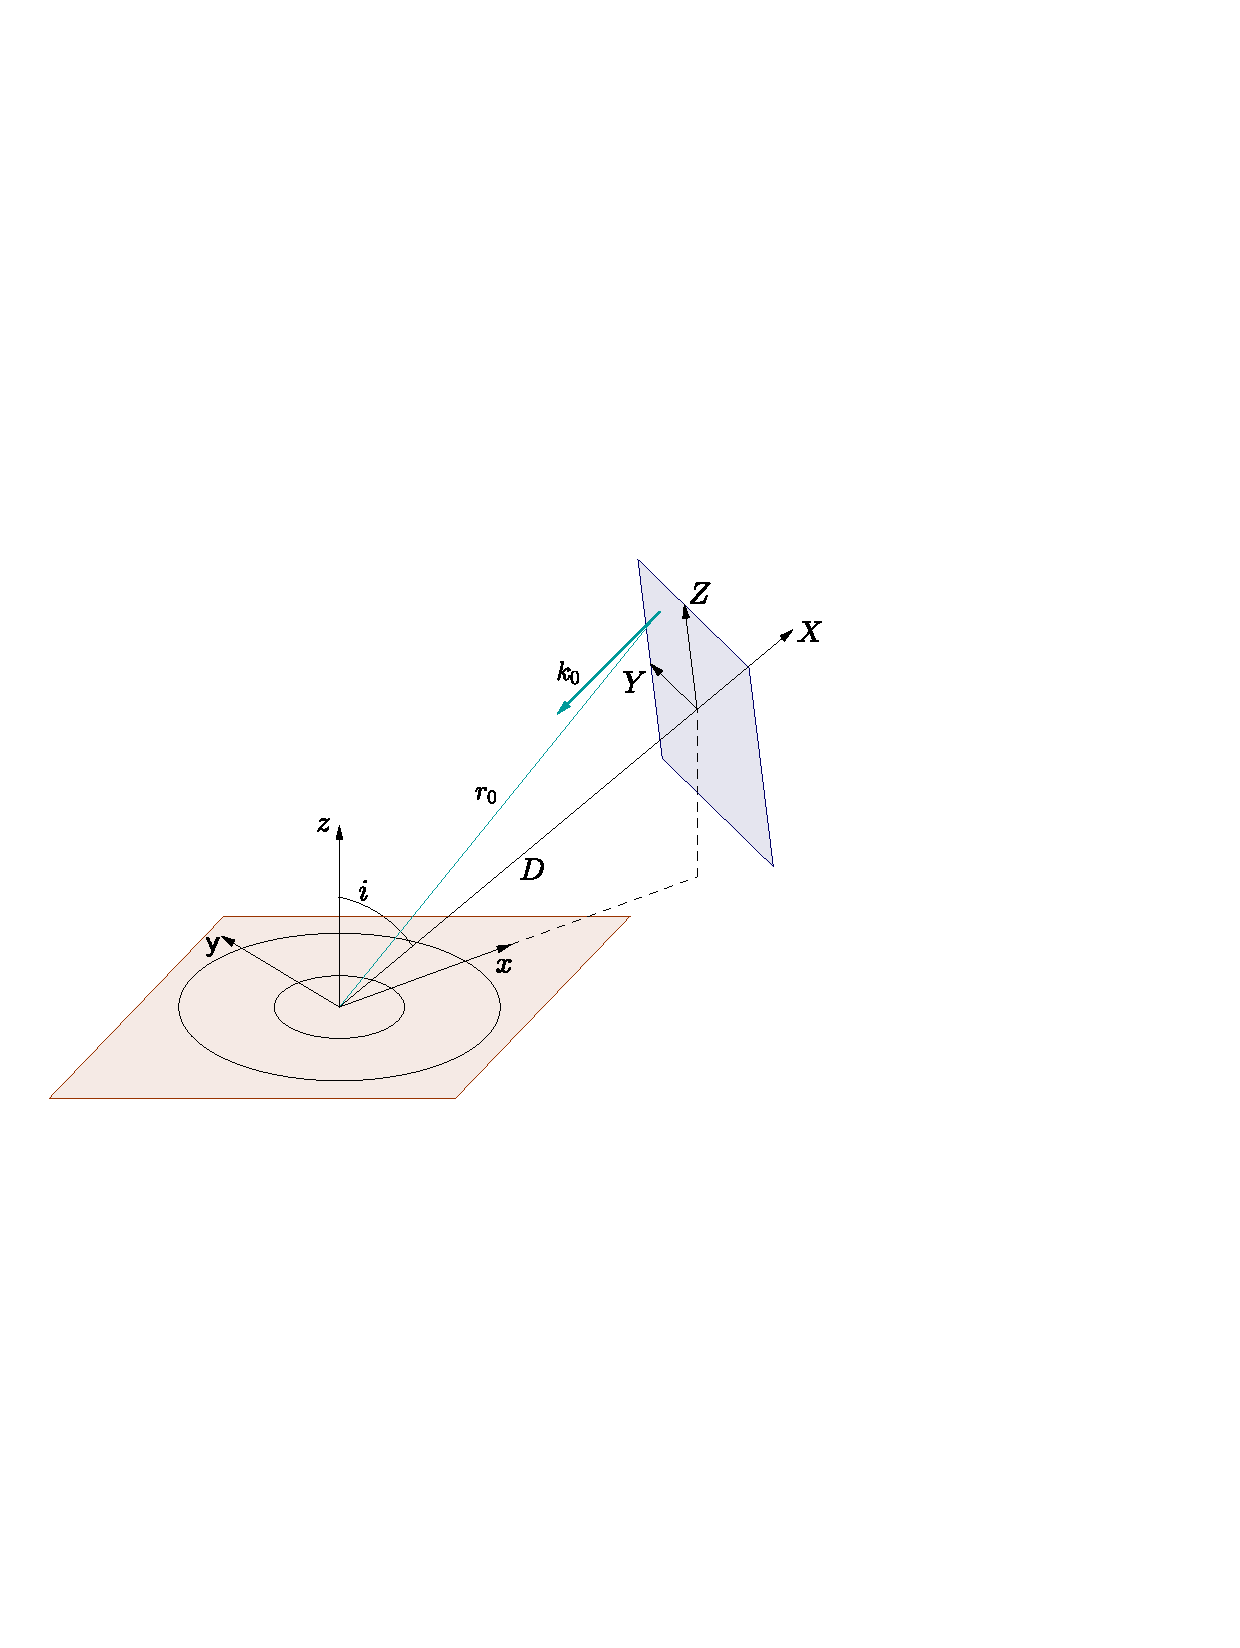
\includegraphics[scale=0.7]{figure01.pdf} 
\caption{Coordinate Transformation relating the observer's system with the black hole's system.}
\label{fig: CoordinateTransformation }
\end{center}
\end{figure}

If the observer is located at a distance $D$ from the black hole as in Figure \ref{fig: CoordinateTransformation }, we introduce the spatial translation from the intermediate system $(X',Y',Z')$ to the system $(x,y,z)$,

\begin{equation}
\begin{pmatrix}
x \\
y \\
z
\end{pmatrix} =\begin{pmatrix}
X' \\
Y' \\
Z'
\end{pmatrix} +
\begin{pmatrix}
D \cos \alpha \\
0 \\
D \sin \alpha
\end{pmatrix}
\end{equation}

The composition of these two transformations give

\begin{equation}
\begin{pmatrix}
x \\
y \\
z
\end{pmatrix} =
\begin{pmatrix}
\cos \alpha & 0 &-\sin\alpha \\
0 & 1 &0\\
\sin \alpha &  0 & \cos \alpha\\
\end{pmatrix} 
\begin{pmatrix}
X\\
Y\\
Z
\end{pmatrix} +
\begin{pmatrix}
D \cos \alpha \\
0 \\
D \sin \alpha
\end{pmatrix}
\end{equation}
or more explicitly,
\begin{equation}
\begin{cases}
x &= X\cos \alpha - Z \sin\alpha + D \cos \alpha\\
y &= Y\\
z &= X \sin \alpha + Z \cos \alpha + D \sin \alpha .\\
\end{cases}
\end{equation}

Since the angle $\alpha$ is related with the inclination angle by $\alpha = \frac{\pi}{2} - i$ we replace the trigonometric functions in the coordinate transformations by
\begin{equation}
\begin{cases}
x &= X\sin i - Z \cos i + D \sin i\\
y &= Y\\
z &= X \cos i + Z \sin i + D \cos i\\
\end{cases}
\end{equation}
or better
\begin{equation}
\begin{cases}
x &= (X+D)\sin i - Z \cos i \\
y &= Y\\
z &= (X+D) \cos i + Z \sin i .\\
\end{cases}
\end{equation}

Since the black hole's metric will be given in spherical coordinates, we introduce the relation between the Cartesian system $(x,y,z)$ and the coordinates $(r,\theta, \phi)$ by

\begin{equation}
\begin{cases}
r &= \sqrt{x^2 + y^2 + z^2} \\
\theta &= \arccos \left( \frac{z}{r}\right)\\
\phi &= \arctan \left( \frac{y}{x} \right) . \\
\end{cases}
\end{equation}

Hence, the complete transformations needed to describe the initial conditions of the photon in spherical coordinates are 

\begin{equation}
\begin{cases}
r &= \sqrt{(X+D)^2 + Y^2 + Z^2} \\
\theta &= \arccos \left( \frac{(X+D) \cos i + Z \sin i}{\sqrt{(X+D)^2 + Y^2 + Z^2}}\right)\\
\phi &= \arctan \left( \frac{Y}{(X+D)\sin i - Z \cos i} \right) . \\
\end{cases} \label{CoordinateTransformation}
\end{equation}

\subsection{Momentum of a Photon}

The Cartesian components of a general incident photon are given by a 4-momentum vector
\begin{equation}
\tilde{k}^\nu_0 =\left( \tilde{k}^t_0, \tilde{k}^X_0, \tilde{k}^Y_0, \tilde{k}^Z_0 \right).
\end{equation}

The components of the 4-momentum in the spherical coordinate system $(r,\theta,\phi)$ are obtained using the transformation law
\begin{equation}
k^\mu = \frac{\partial x^\mu}{\partial \tilde{x}^\nu} \tilde{k}^\nu.
\label{kTransformation}
\end{equation}



\section{Image Plane Screen}

The observer's image plane is considered as a grid located at a distant point and we will consider photons received there with  a momentum vector which is orthogonal to the  plane. The algorithm will evolve the trajectories back in time onto the emission structure around the black hole. 

\subsection{Initial Position of a photon}

Consider a photon registered at the observer's image plane at the coordinates $(X,Y,Z) = (0, \alpha, \beta)$ at the time $t_0 = 0$. The spherical coordinates of this photon as seen from the black hole are given by the equation (\ref{CoordinateTransformation}) as

\begin{equation}
\begin{cases}
t_0 &= 0\\
r_0 &= \sqrt{D^2 + \alpha^2 + \beta^2} \\
\theta_0 &= \arccos \left( \frac{D \cos i + \beta \sin i}{\sqrt{D^2 + \alpha^2 + \beta^2}}\right)\\
\phi_0 &= \arctan \left( \frac{\alpha}{D\sin i - \beta \cos i} \right) \\
\end{cases} 
\end{equation}

\subsection{Momentum of a Photon}

Photons received by the distant observer will be considered to arrive perpendicular to the image plane. According to the orientation of the coordinates $(X,Y,Z)$ in Figure \ref{fig: CoordinateTransformation }, the Cartesian components of the incident photon are given by
\begin{equation}
\tilde{k}^\nu_0 =\left( \tilde{k}^t_0, \tilde{k}^X_0, \tilde{k}^Y_0, \tilde{k}^Z_0 \right) = \left( K_0, K_0, 0, 0 \right).
\end{equation}

The components of the 4-momentum in the spherical coordinate system  are obtained using  Eq. (\ref{kTransformation}). Given the perpendicular components of the incident photon, the relevant terms in the transformation matrix are obtained from equation (\ref{CoordinateTransformation}) as

\begin{equation}
\left. \frac{\partial r}{\partial X} \right|_{(0,\alpha,\beta)}= \left.\frac{X+D}{\sqrt{(X+D)^2 + Y^2 + Z^2}}\right|_{(0,\alpha,\beta)}
= \frac{D}{\sqrt{D^2 + \alpha^2 + \beta^2}} = \frac{D}{r_0}
\end{equation}

\footnotesize
\begin{equation}
\left. \frac{\partial \theta}{\partial X} \right|_{(0,\alpha,\beta)} = \left.-\frac{1}{\sqrt{r^2-[(X+D)\cos i + Z \sin i]^2}}  \left[ \cos i - \frac{(X+D)^2 \cos i + Z(X+D) \sin i}{r^2}\right]\right|_{(0,\alpha,\beta)} \nonumber
\end{equation}
\normalsize

\begin{equation}
\left. \frac{\partial \theta}{\partial X} \right|_{(0,\alpha,\beta)} = -\frac{1}{\sqrt{r^2_0 -[D\cos i + \beta \sin i]^2}}  \left[ \cos i - \frac{D^2 \cos i + D\beta \sin i}{r^2_0}\right]\\
\end{equation}

\begin{align}
\left. \frac{\partial \phi}{\partial X} \right|_{(0,\alpha,\beta)} &= \left.-\frac{Y \sin i}{[(X+D)\sin i - Z \cos i ]^2 + Y^2 } \right|_{(0,\alpha,\beta)} \nonumber \\
\left. \frac{\partial \phi}{\partial X} \right|_{(0,\alpha,\beta)} &= -\frac{\alpha \sin i}{\alpha^2 +[D \sin i - \beta \cos i]^2 }  
\end{align}

Hence, the spatial components of the initial 4-momentum in spherical coordinates are

\begin{equation}
\begin{cases}
k^r_0 &= \frac{D}{r_0} K_0\\
k^\theta _0 &= -\frac{1}{\sqrt{\alpha^2 +[D\sin i - \beta \cos i]^2}}  \left[ \cos i - \frac{D^2 \cos i + D\beta \sin i}{r^2_0}\right] K_0 \\
k^\phi _0 &= -\frac{\alpha \sin i}{\alpha^2 +[D \sin i - \beta \cos i]^2 } K_0
\end{cases} \label{initialSpatialMomentum}
\end{equation}

The temporal component of the initial 4-momentum of the photon is obtained from the condition 
\begin{equation}
k^\mu k_\mu =  \eta_{\mu \nu} k^\mu k^\nu = 0,
\end{equation}
which gives
\begin{equation}
k^t_0 = \sqrt{(k^r_0)^2 + r_0^2 (k^\theta _0)^2 + r_0^2 \sin^2 \theta_0 (k^\phi _0)^2}. \label{initialTempMomentum}
\end{equation}


\subsection{Complete Set of Initial Conditions}

The complete set of initial conditions are given by equations (\ref{CoordinateTransformation}), (\ref{initialSpatialMomentum}) and (\ref{initialTempMomentum}),

\begin{align}
t_0 &= 0\\
r_0 &= \sqrt{D^2 + \alpha^2 + \beta^2} \\
\theta_0 &= \arccos \left( \frac{D \cos i + \beta \sin i}{\sqrt{D^2 + \alpha^2 + \beta^2}}\right)\\
\phi_0 &= \arctan \left( \frac{\alpha}{D\sin i - \beta \cos i} \right) \\
k^t_0 &= \sqrt{(k^r_0)^2 + r_0^2 (k^\theta _0)^2 + r_0^2 \sin^2 \theta_0 (k^\phi _0)^2}\\
k^r_0 &= \frac{D}{r_0} K_0\\
k^\theta _0 &= -\frac{1}{\sqrt{\alpha^2 +[D\sin i - \beta \cos i]^2}}  \left[ \cos i - \frac{D^2 \cos i + D\beta \sin i}{r^2_0}\right] K_0 \\
k^\phi _0 &= -\frac{\alpha \sin i}{\alpha^2 +[D \sin i - \beta \cos i]^2 } K_0
\end{align}


\section{Point Camera}

Another type of screen considered in this project is a point camera. Photons arrive to this point receptor  from different directions. Therefore, in this case the initial position of all photon in the image is the same (point camera) while the components of the initial 4-momentum vector distinguishes each photon.

\subsection{Initial Position of a photon}

Since all the photons arrive to one point, the initial position condition for any of the photons is just $(X,Y,Z) = (0,0,0)$ at the time $t_0 = 0$. The corresponding spherical coordinates as seen from the black hole are given by the equations (\ref{CoordinateTransformation}),

\begin{equation}
\begin{cases}
t_0 &= 0\\
r_0 &= D\\
\theta_0 &= i \\
\phi_0 &= 0 \\
\end{cases} 
\end{equation}

\subsection{Momentum of a Photon}

Photons arrive to the point camera from different directions. Using the angular coordinates $\alpha$ and $\beta$ to describe the direction of each photon, the cartesian components of the 4-momentum vector can be written as
\begin{equation}
\tilde{k}^\nu_0 =\left( \tilde{k}^t_0, \tilde{k}^X_0, \tilde{k}^Y_0, \tilde{k}^Z_0 \right) = \left( K_0, K_0 \cos \beta \cos \alpha , K_0 \cos \beta \sin \alpha , K_0 \sin \beta \right).
\end{equation}

The components of the 4-momentum in the spherical coordinate system  are obtained using  Eq. (\ref{kTransformation}). The relevant terms in the transformation matrix are obtained from equation (\ref{CoordinateTransformation}) evaluating at the position of the point camera, giving

\begin{equation}
\left. \frac{\partial r}{\partial X} \right|_{(0,0,0)}= \left.\frac{X+D}{\sqrt{(X+D)^2 + Y^2 + Z^2}}\right|_{(0,0,0)}
= \frac{D}{\sqrt{D^2}} = 1
\end{equation}

\begin{equation}
\left. \frac{\partial r}{\partial Y} \right|_{(0,0,0)}= \left.\frac{Y}{\sqrt{(X+D)^2 + Y^2 + Z^2}}\right|_{(0,0,0)} = 0
\end{equation}

\begin{equation}
\left. \frac{\partial r}{\partial Z} \right|_{(0,0,0)}= \left.\frac{Z}{\sqrt{(X+D)^2 + Y^2 + Z^2}}\right|_{(0,0,0)} = 0
\end{equation}

\footnotesize
\begin{align}
\left. \frac{\partial \theta}{\partial X} \right|_{(0,0,0)} &= \left.-\frac{1}{\sqrt{r^2-[(X+D)\cos i + Z \sin i]^2}}  \left[ \cos i - \frac{(X+D)^2 \cos i + Z(X+D) \sin i}{r^2}\right]\right|_{(0,0,0)} \nonumber \\
\left. \frac{\partial \theta}{\partial X} \right|_{(0,0,0)} &= -\frac{1}{\sqrt{D^2 -[D\cos i ]^2}}  \left[ \cos i - \frac{D^2 \cos i }{D^2}\right]=0
\end{align}
\normalsize

\footnotesize
\begin{align}
\left. \frac{\partial \theta}{\partial Y} \right|_{(0,0,0)} &= \left.-\frac{1}{\sqrt{r^2-[(X+D)\cos i + Z \sin i]^2}}  \left[ -Y \frac{(X+D) \cos i + Z \sin i}{r^2}\right]\right|_{(0,0,0)} \nonumber \\
\left. \frac{\partial \theta}{\partial Y} \right|_{(0,0,0)} &=0
\end{align}
\normalsize

\footnotesize
\begin{align}
\left. \frac{\partial \theta}{\partial Z} \right|_{(0,0,0)} &= \left.-\frac{1}{\sqrt{r^2-[(X+D)\cos i + Z \sin i]^2}}  \left[ \sin i -  Z \frac{(X+D) \cos i + Z \sin i}{r^2}\right]\right|_{(0,0,0)} \nonumber \\
\left. \frac{\partial \theta}{\partial Z} \right|_{(0,0,0)} &= -\frac{\sin i}{\sqrt{D^2 -[D\cos i ]^2}} = - \frac{1}{D}
\end{align}
\normalsize

\begin{align}
\left. \frac{\partial \phi}{\partial X} \right|_{(0,0,0)} &= \left.-\frac{Y \sin i}{[(X+D)\sin i - Z \cos i ]^2 + Y^2 } \right|_{(0,0,0)} \nonumber \\
\left. \frac{\partial \phi}{\partial X} \right|_{(0,0,0)} &= 0  
\end{align}

\begin{align}
\left. \frac{\partial \phi}{\partial Y} \right|_{(0,0,0)} &= \left.\frac{[(X+D)\sin i - Z \cos i ]}{[(X+D)\sin i - Z \cos i ]^2 + Y^2 } \right|_{(0,0,0)} \nonumber \\
\left. \frac{\partial \phi}{\partial Y} \right|_{(0,0,0)} &= \frac{D \sin i  }{[D \sin i ]^2 }  = \frac{1}{ D \sin i  }
\end{align}

\begin{align}
\left. \frac{\partial \phi}{\partial Z} \right|_{(0,0,0)} &= \left.\frac{Y \cos i}{[(X+D)\sin i - Z \cos i ]^2 + Y^2 } \right|_{(0,0,0)} \nonumber \\
\left. \frac{\partial \phi}{\partial Z} \right|_{(0,0,0)} &= 0  
\end{align}

Using this components of the transformation matrix, the spatial components of the initial 4-momentum in spherical coordinates are

\begin{equation}
\begin{cases}
k^r_0 &= \tilde{k}^X_0 = K_0 \cos \beta \cos \alpha  \\
k^\theta _0 &= \left. \frac{\partial \theta}{\partial Z} \right|_{(0,0,0)}  \tilde{k}^Z_0 = - \frac{K_0 \sin \beta}{D} \\
k^\phi _0 &= \left. \frac{\partial \phi}{\partial Y} \right|_{(0,0,0)}  \tilde{k}^Y_0 = \frac{K_0 \cos \beta \sin \alpha}{ D \sin i  }
\end{cases} \label{initialSpatialMomentum2}
\end{equation}

The temporal component of the initial 4-momentum of the photon is obtained from the condition 
\begin{equation}
k^\mu k_\mu =  \eta_{\mu \nu} k^\mu k^\nu = 0,
\end{equation}
which gives
\begin{equation}
k^t_0 = \sqrt{(k^r_0)^2 + r_0^2 (k^\theta _0)^2 + r_0^2 \sin^2 \theta_0 (k^\phi _0)^2}. \label{initialTempMomentum2}
\end{equation}

\section{Covariant Components of the 4-Momentum Vector}
In order to solve the Hamiltonian equations of motion for the photons, we will need the initial components of the 4-momentum vector in their covariant form. Therefore we need to apply the spacetime metric $g_{\mu \nu}$ as
\begin{equation}
k_\mu = g_{\mu \nu} k^\nu.
\end{equation}

For a general stationary and axially symmetric spacetime described with the line element
\begin{equation}
ds^2 = g_{tt} dt^2 + 2g_{t \phi} dt d\phi + g_{rr} dr^2 + g_{\theta \theta} d\theta^2 + g_{\phi \phi} d\phi^2
\end{equation}
the covariant components of the 4-momentum are
\begin{equation}
\begin{cases}
k_t &= g_{tt} k^t + g_{t \phi} k^\phi\\
k_r &= g_{rr} k^r \\
k_\theta &= g_{\theta \theta} k^\theta \\
k_\phi &=  g_{t \phi} k^t + g_{\phi \phi} k^\phi\\
\end{cases}
\end{equation}